\section{Lancer le syst\`eme d'urgence}Si vous voulez d\'emarrer un poste client en vue de r\'eparation ou de diagnose, vous pouvez d\'emarrer le syst\`eme d'urgence par le r\'eseau. Apr\`es le d\'emarrage, le client lance une console sur laquelle vous pouvez travailler. Pour lancer le syst\`eme d'urgence, cliquez sur \textit{$\ll$Syst�me d'urgence$\gg$} derri\`ere le nom du client.\\
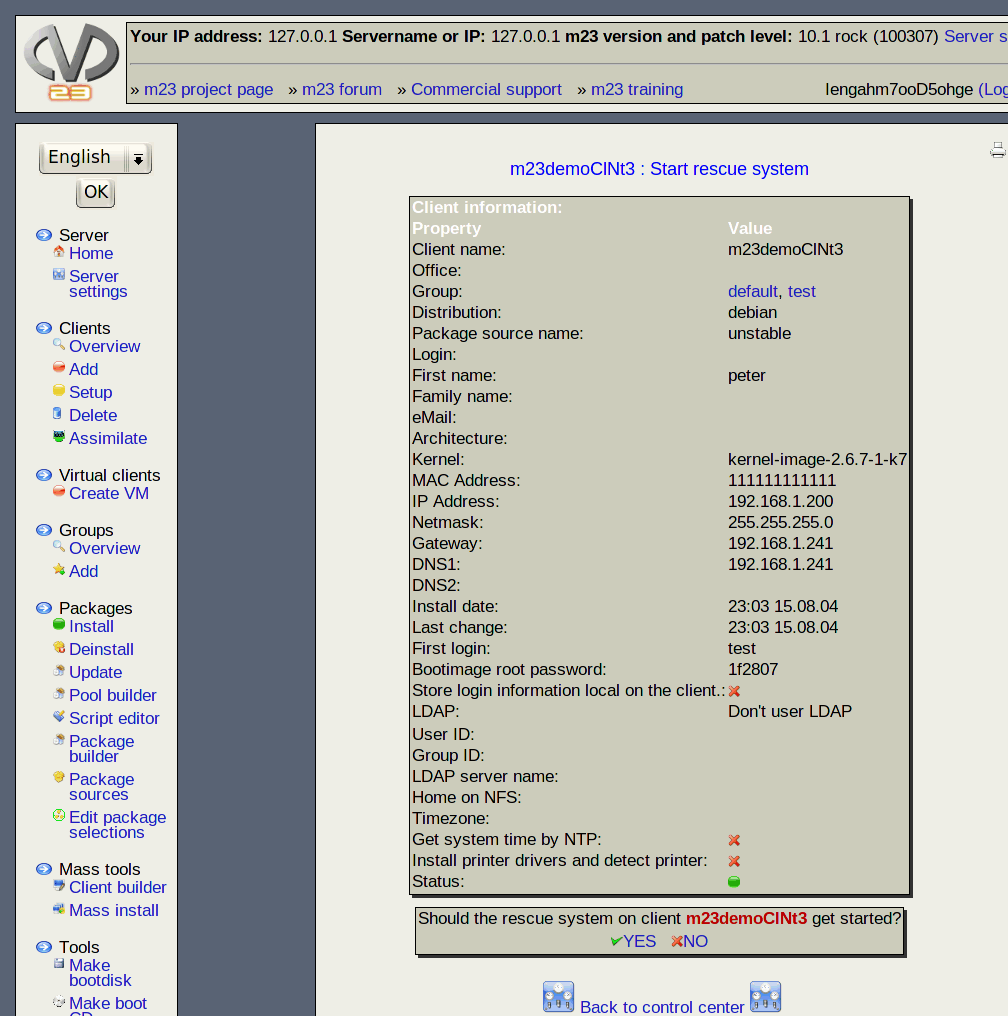
\includegraphics[scale=0.4]{/mdk/doc/manual/screenshots/fr/rescue_client.png} \\
\subsection{Notez}
Le syst\`eme d'urgence sera lanc\'e chaque fois apr\`es le d\'emarrage jusqu'\`a ce que vous effaciez la t\^ache de la liste des travaux. Vous la trouvez en cliquant sur le num\'ero dans la colonne \textit{$\ll$Travaux$\gg$} de la page \textit{$\gg$Vue d'ensemble des postes clients$\gg$}.\\
